
\begin{figure}[H]
\centering
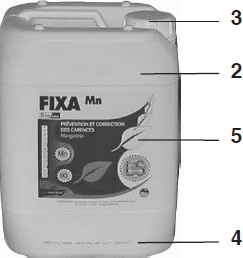
\includegraphics[width=.45\linewidth]{fig_00.png}
%\caption{ \label{fig_}}
\end{figure}


\begin{figure}[H]
\centering
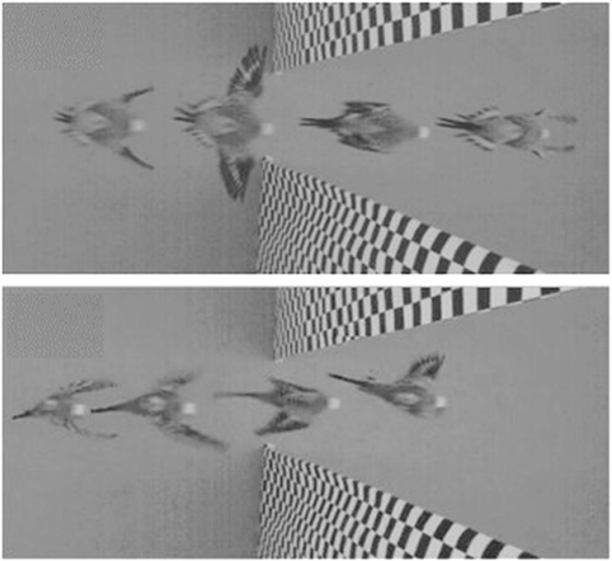
\includegraphics[width=.45\linewidth]{fig_01.png}
\caption{Détection par ultrasons (4 capteurs) \label{fig_01}}
\end{figure}


\begin{figure}[H]
\centering
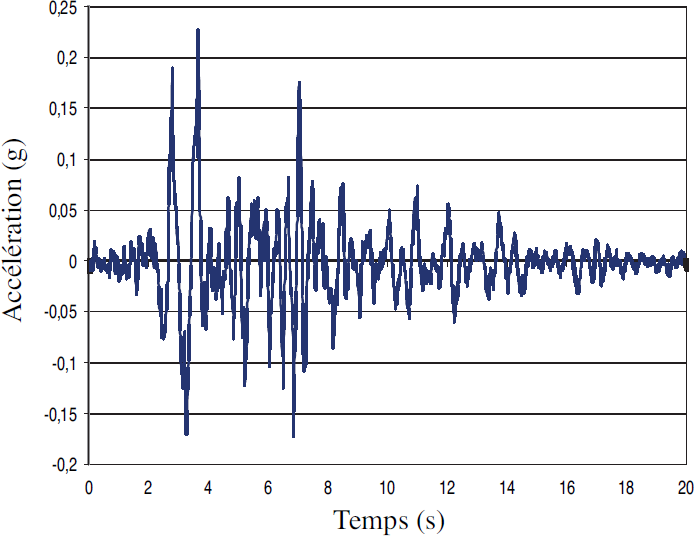
\includegraphics[width=.45\linewidth]{fig_02.png}
\caption{Manoeuvre d’insertion en créneau dans une place de stationnement \label{fig_02}}
\end{figure}


\begin{figure}[H]
\centering
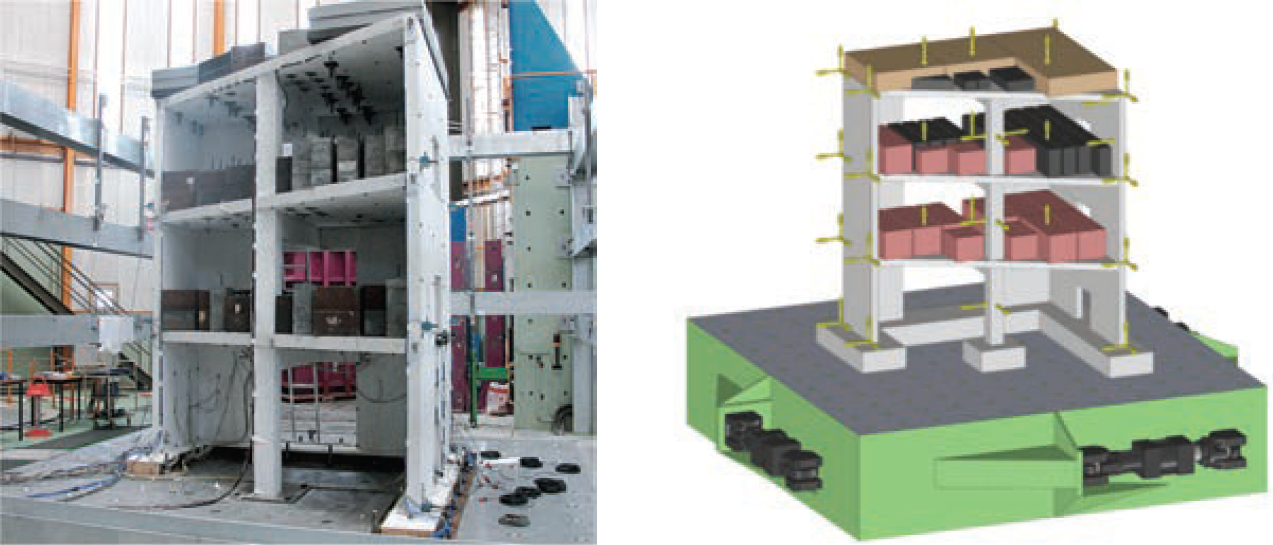
\includegraphics[width=.45\linewidth]{fig_03.png}
\caption{Phase de détection d’une place libre \label{fig_03}}
\end{figure}


\begin{figure}[H]
\centering
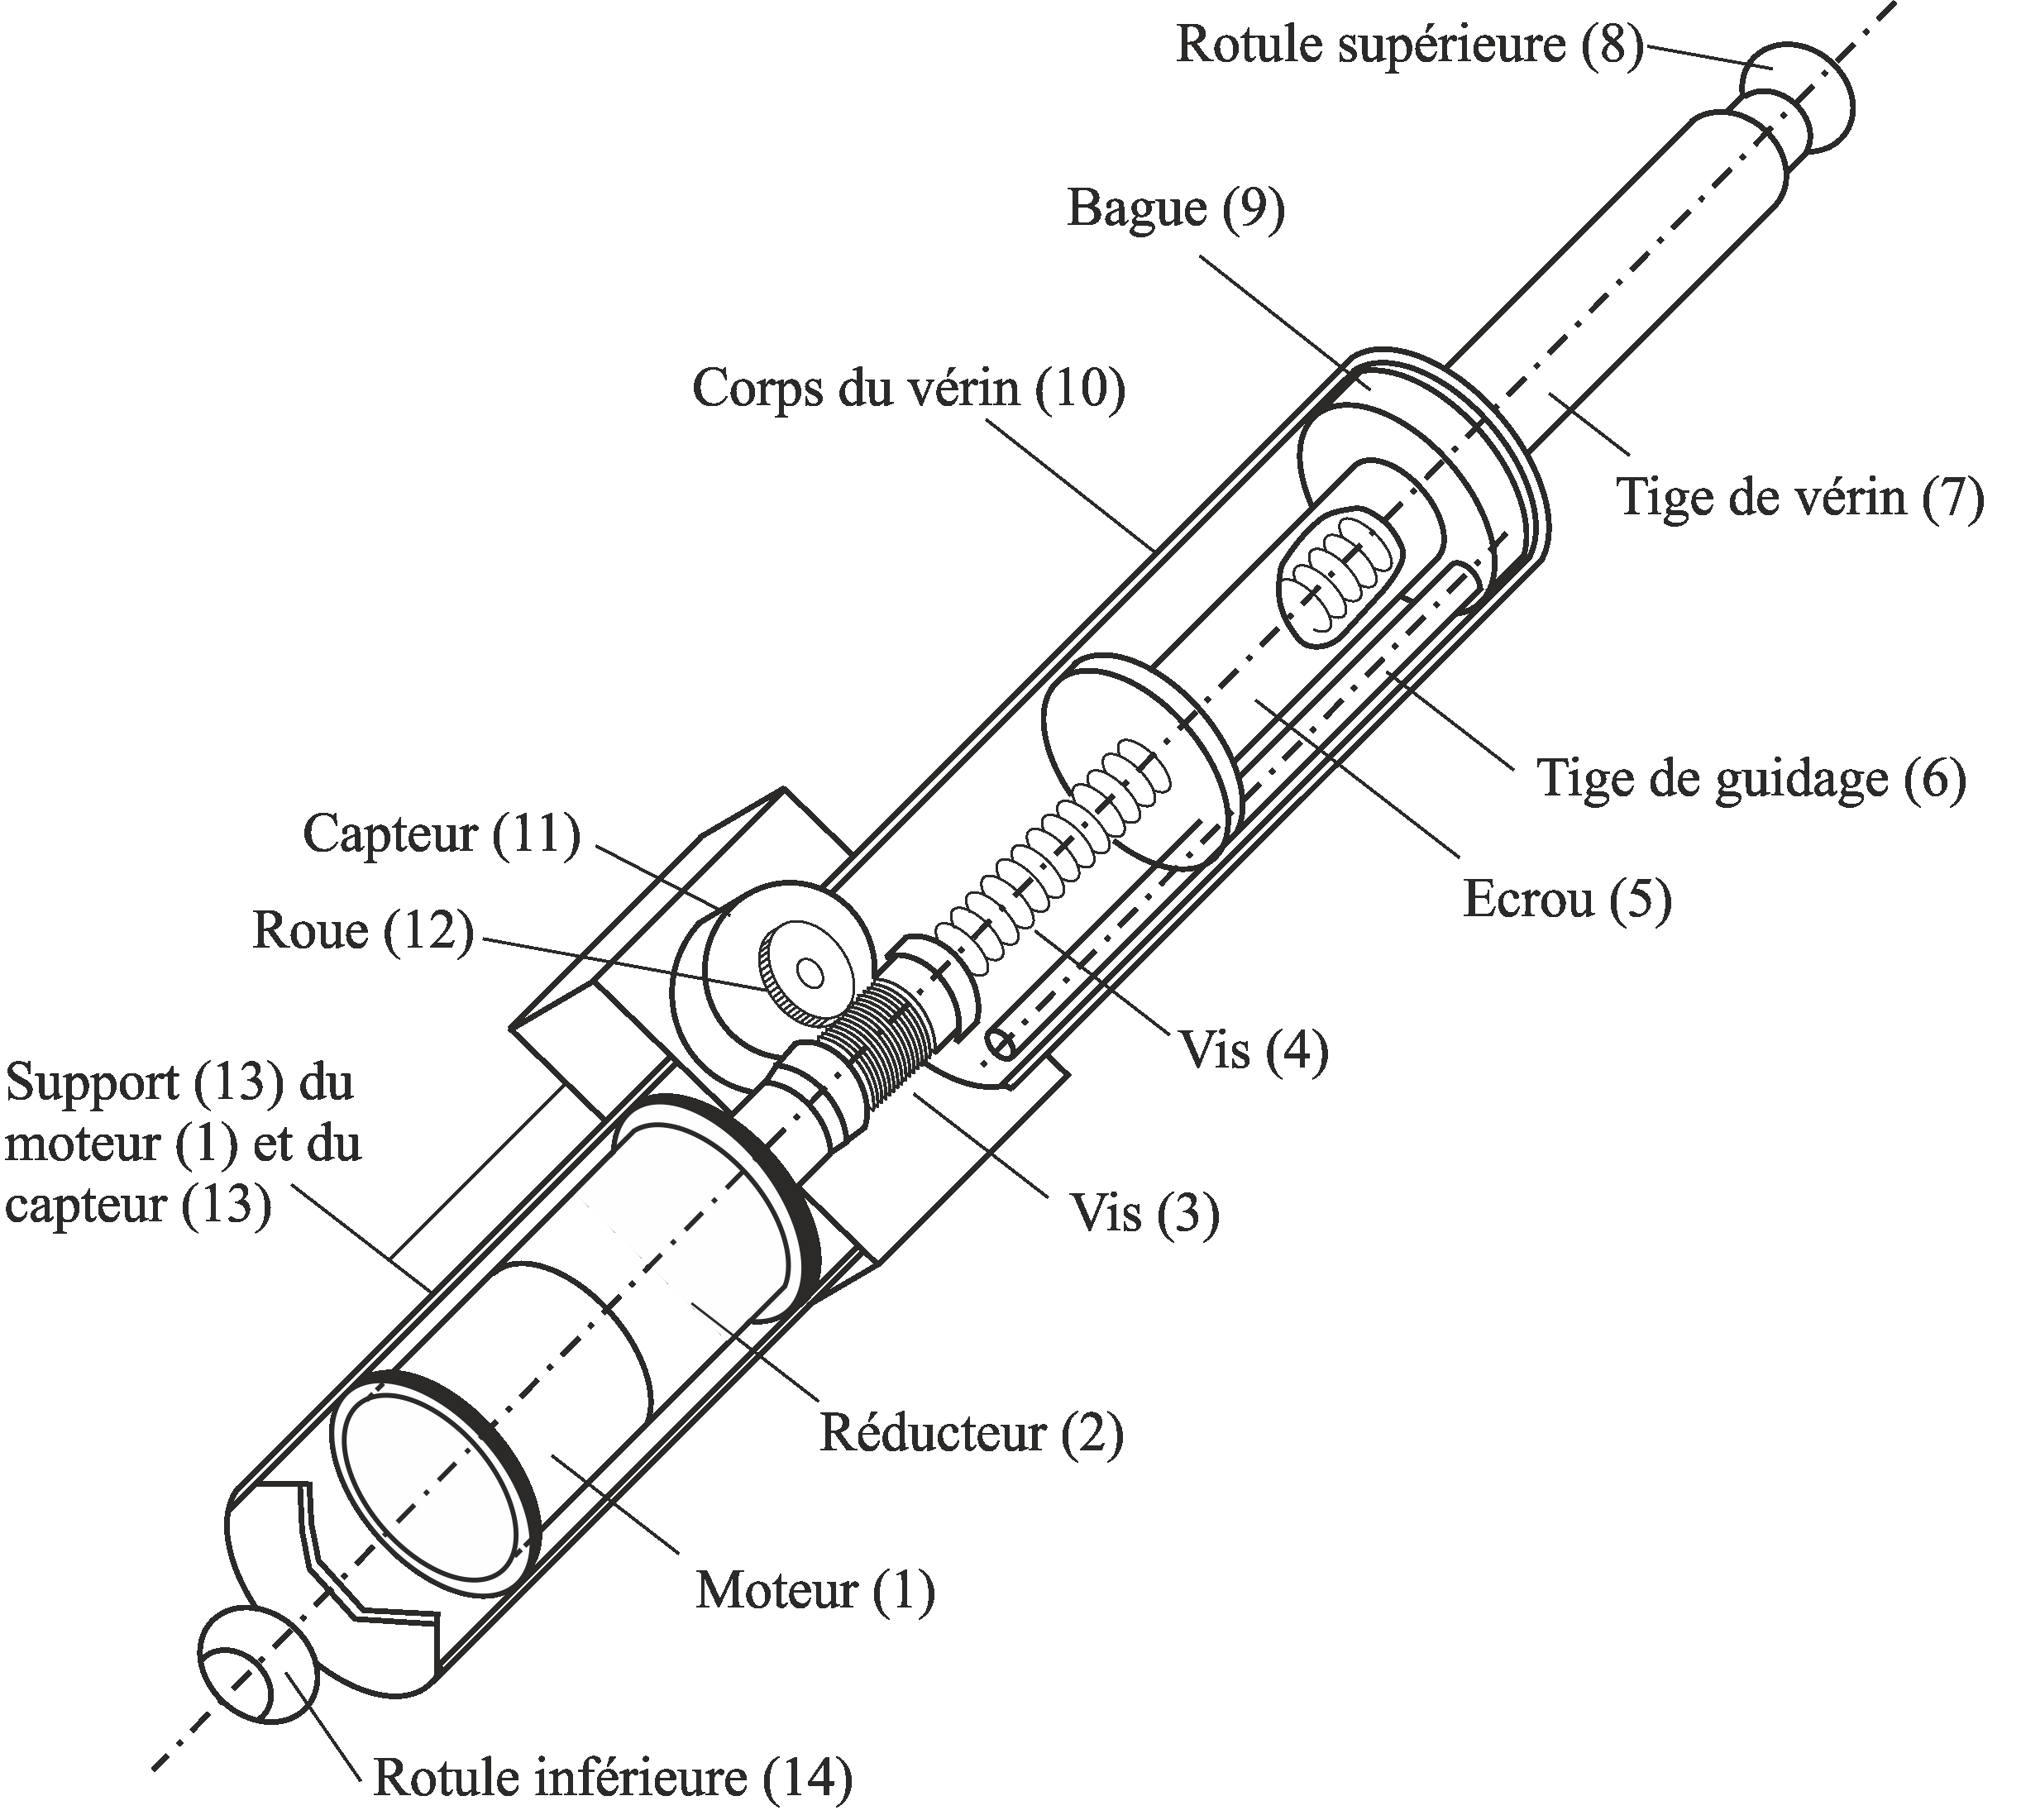
\includegraphics[width=.45\linewidth]{fig_04.png}
\caption{Principe du capteur de proximité \label{fig_04}}
\end{figure}


\begin{figure}[H]
\centering
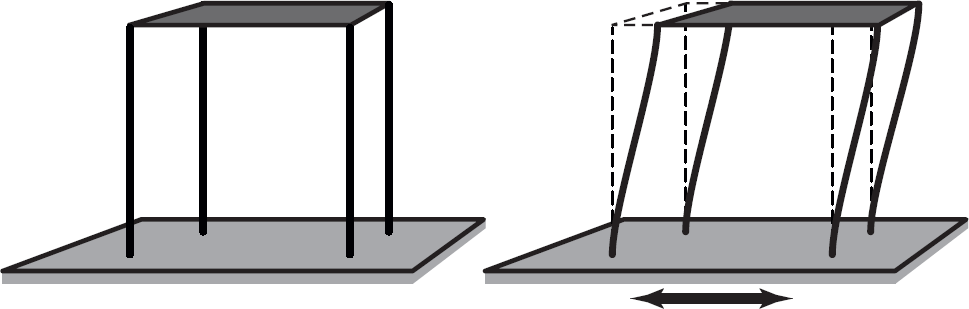
\includegraphics[width=.45\linewidth]{fig_05.png}
\caption{Profil de vitesse du véhicule lors des phases 1, 2 et 3 de la figure \ref{fig_05} \label{fig_05}}
\end{figure}


\begin{figure}[H]
\centering
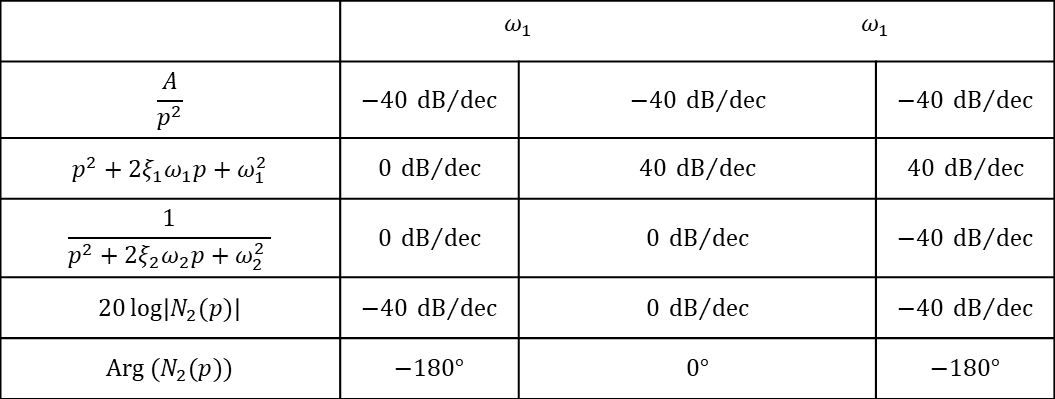
\includegraphics[width=.45\linewidth]{fig_06.png}
\caption{Trajectoire à suivre pour la manoeuvre \label{fig_06}}
\end{figure}


\begin{figure}[H]
\centering
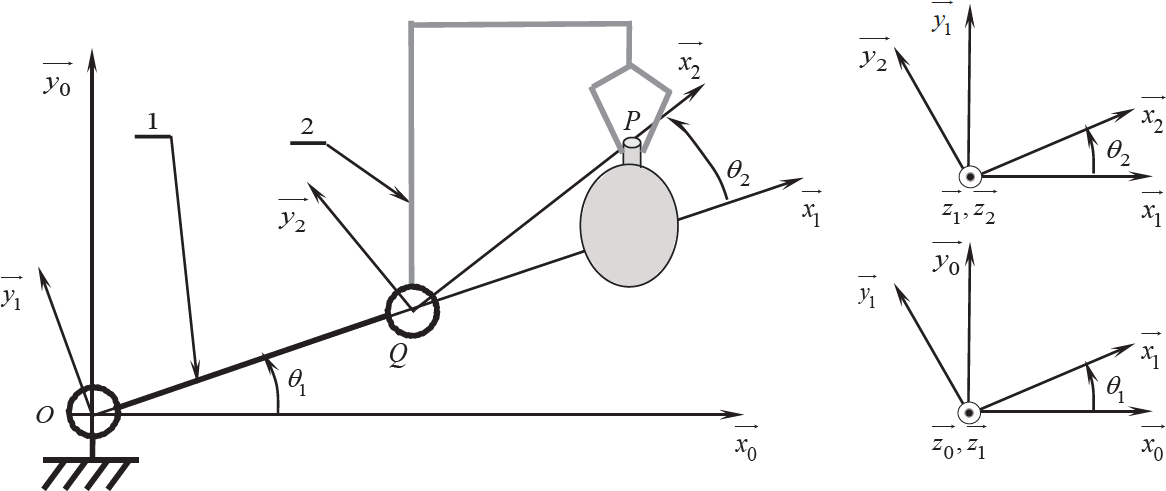
\includegraphics[width=.45\linewidth]{fig_07.png}
\caption{Trajectoire du point $F$ lors de l’insertion dans la place vacante \label{fig_07}}
\end{figure}


\begin{figure}[H]
\centering
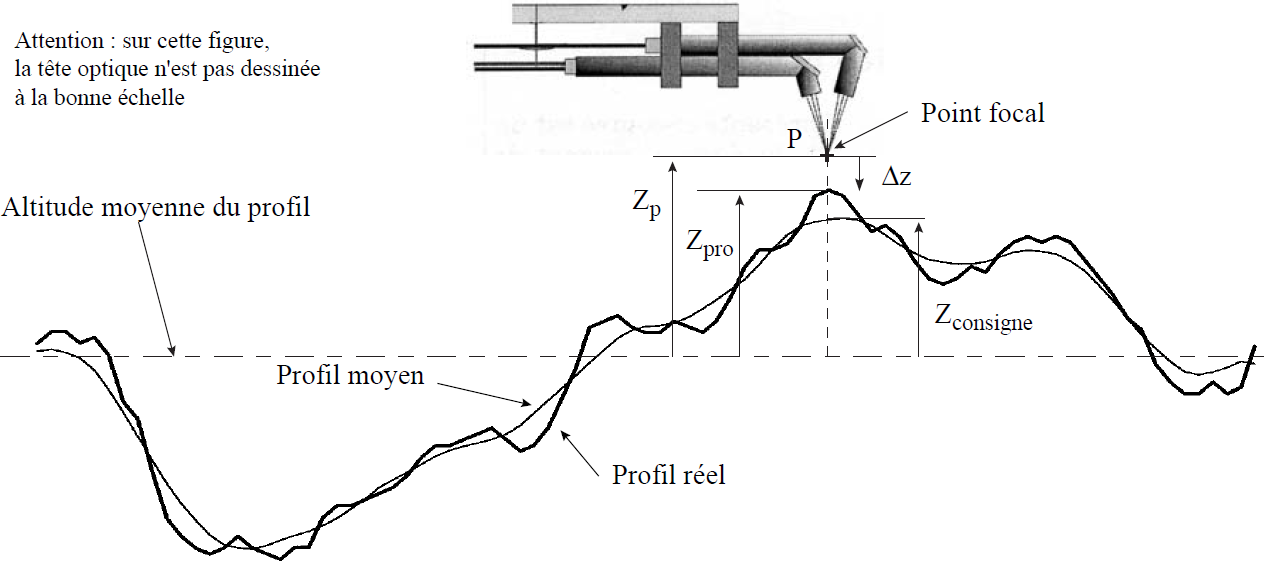
\includegraphics[width=.45\linewidth]{fig_08.png}
\caption{Simulation du stationnement \label{fig_08}}
\end{figure}


\begin{figure}[H]
\centering
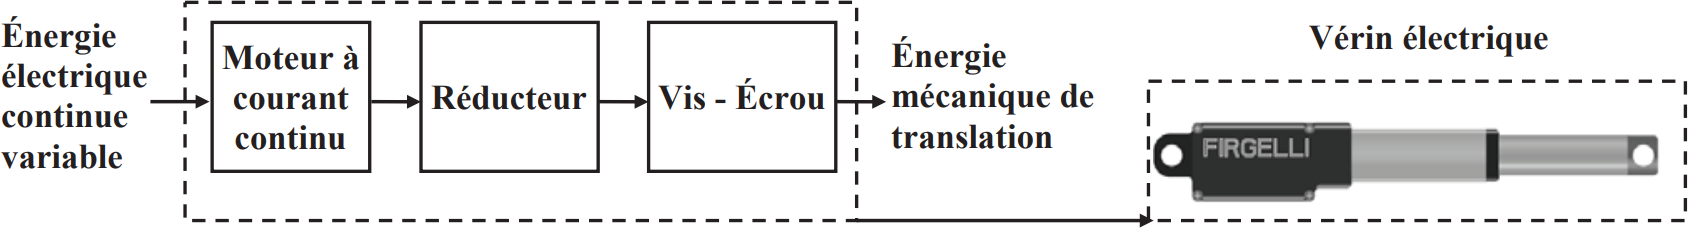
\includegraphics[width=.45\linewidth]{fig_09.png}
\caption{Paramétrage lors de la manoeuvre \label{fig_09}}
\end{figure}


\begin{figure}[H]
\centering
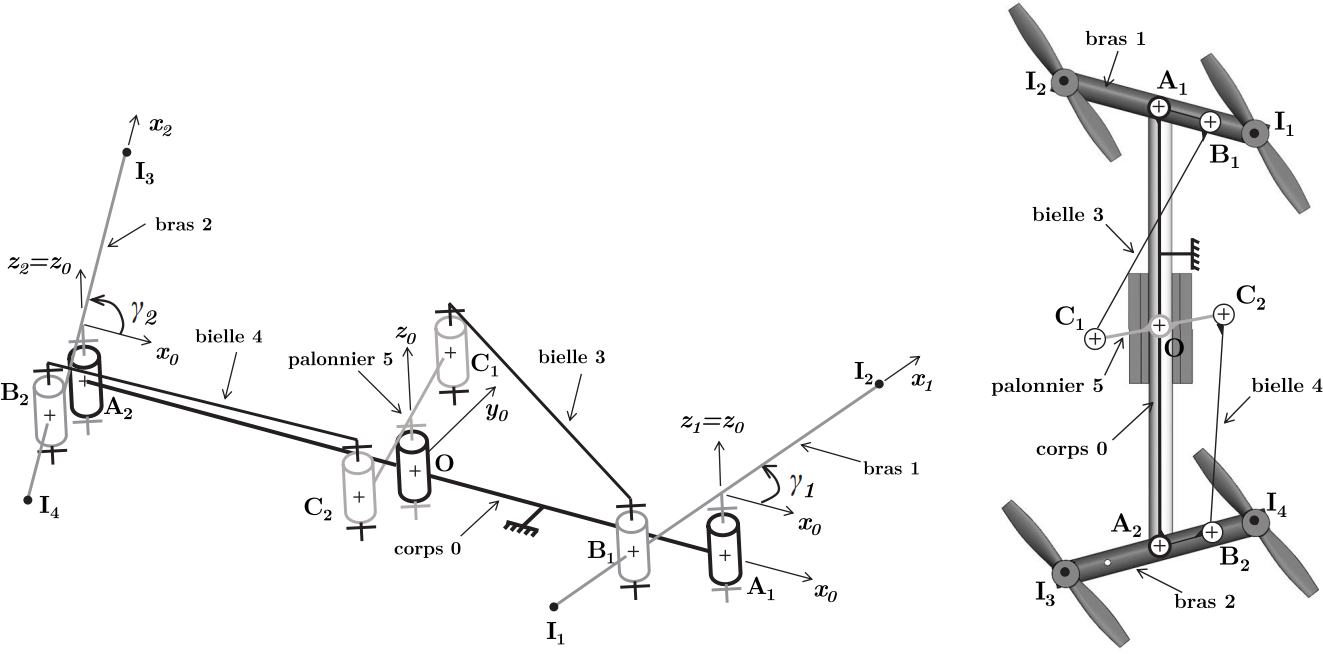
\includegraphics[width=.45\linewidth]{fig_10.png}
\caption{Tamiya M-05 Mazda \label{fig_10}}
\end{figure}


\begin{figure}[H]
\centering
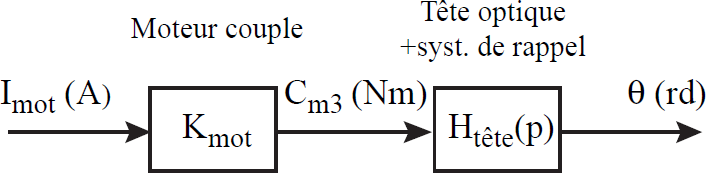
\includegraphics[width=.45\linewidth]{fig_11.png}
\caption{Description chaine d’énergie / chaine d’information de la direction \label{fig_11}}
\end{figure}


\begin{figure}[H]
\centering
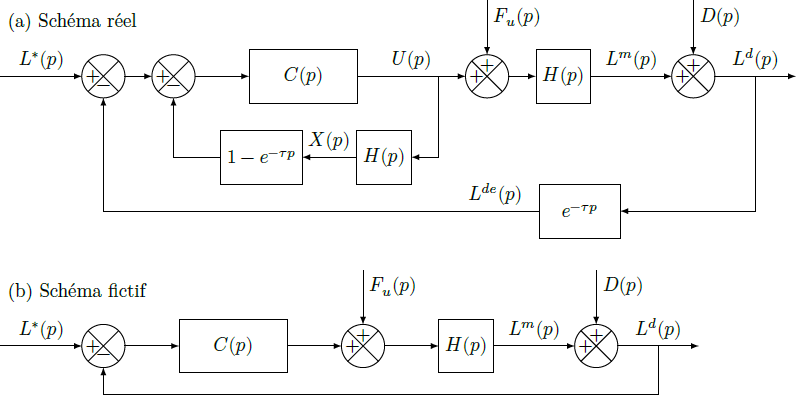
\includegraphics[width=.45\linewidth]{fig_12.png}
\caption{Schéma blocs de la commande en position des roues directrices du véhicule RC \label{fig_12}}
\end{figure}


\begin{figure}[H]
\centering
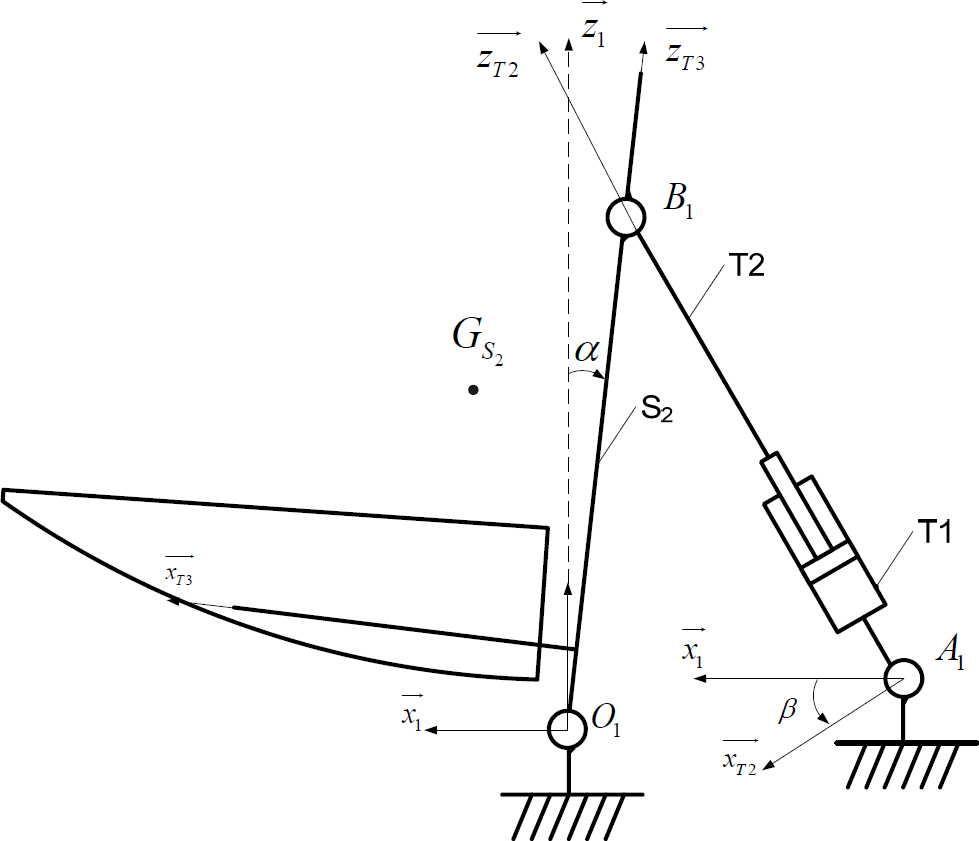
\includegraphics[width=.45\linewidth]{fig_13.png}
\caption{Schéma cinématique plan de la direction du véhicule radio commandé \label{fig_13}}
\end{figure}


\begin{figure}[H]
\centering
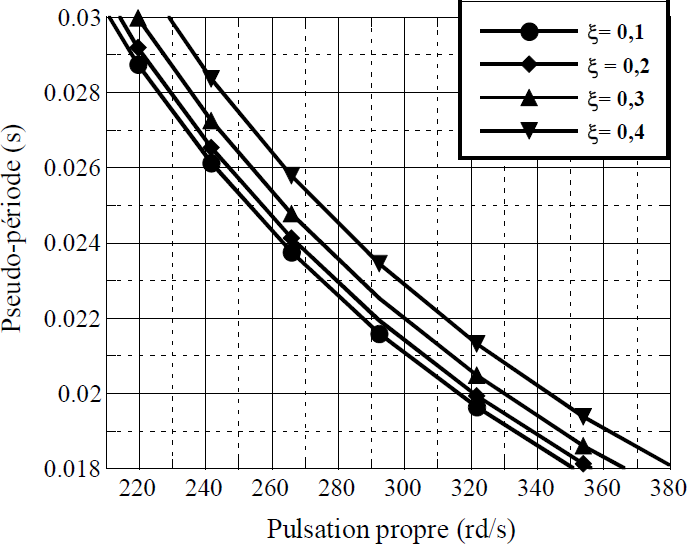
\includegraphics[width=.45\linewidth]{fig_14.png}
\caption{Schéma cinématique plan de la direction du véhicule radio commandé \label{fig_14}}
\end{figure}


\begin{figure}[H]
\centering
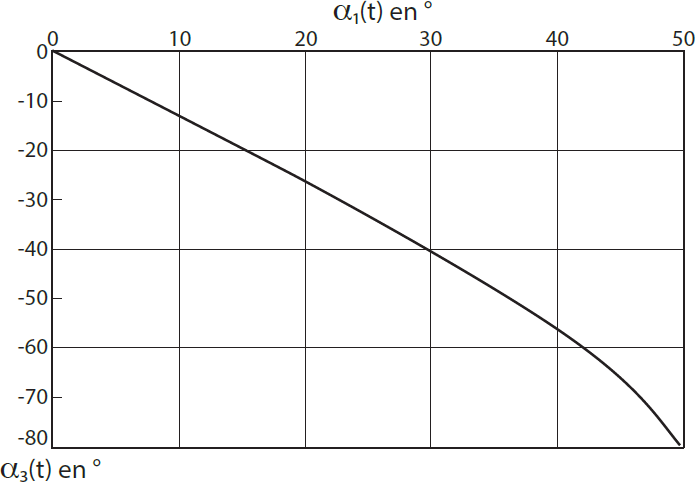
\includegraphics[width=.45\linewidth]{fig_15.png}
\caption{Tracé de $\alpha_3(t)$ en fonction de $\alpha_1(t)$ \label{fig_15}}
\end{figure}


\begin{figure}[H]
\centering
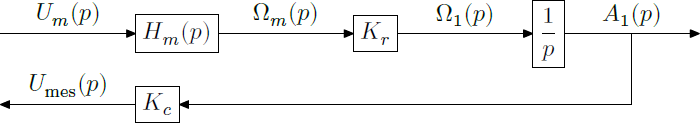
\includegraphics[width=.45\linewidth]{fig_16.png}
\caption{Schéma-blocs du servomoteur seul \label{fig_16}}
\end{figure}


\begin{figure}[H]
\centering
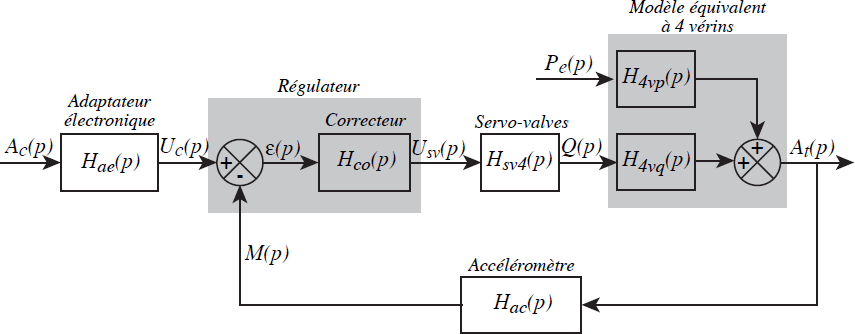
\includegraphics[width=.45\linewidth]{fig_17.png}
\caption{Tension fournie par le potentiomètre du servomoteur pour un échelon de tension $u_m(t)=\SI{3}{V}$ \label{fig_17}}
\end{figure}


\begin{figure}[H]
\centering
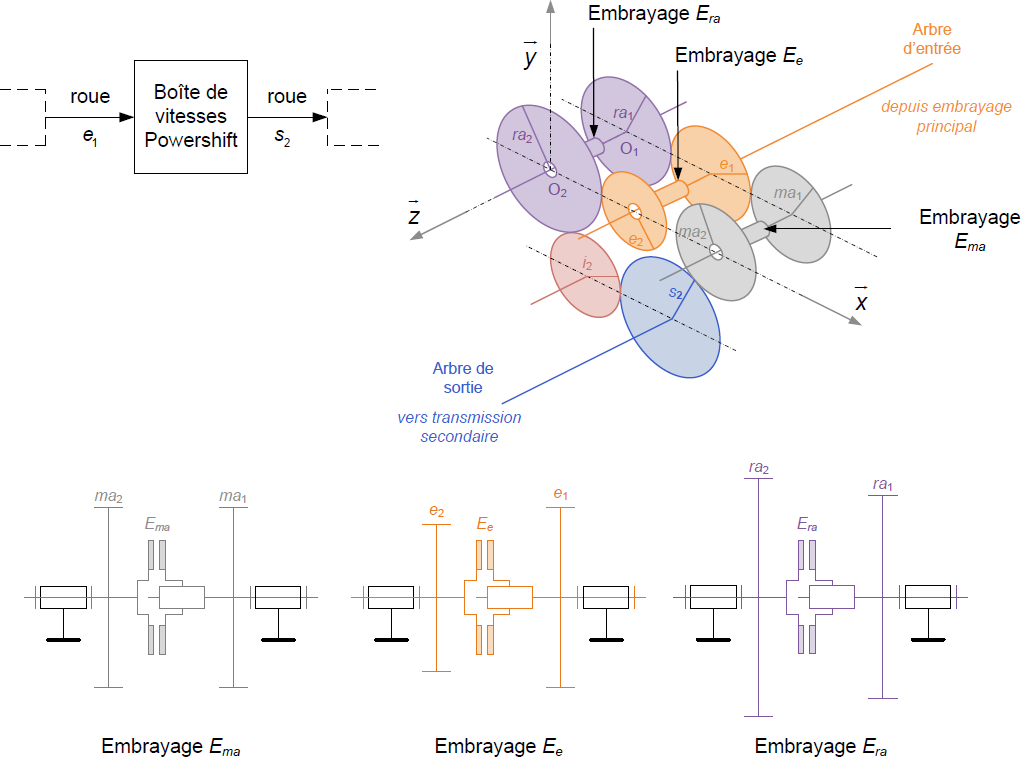
\includegraphics[width=.45\linewidth]{fig_18.png}
\caption{ Intensité moteur\label{fig_18}}
\end{figure}


\begin{figure}[H]
\centering
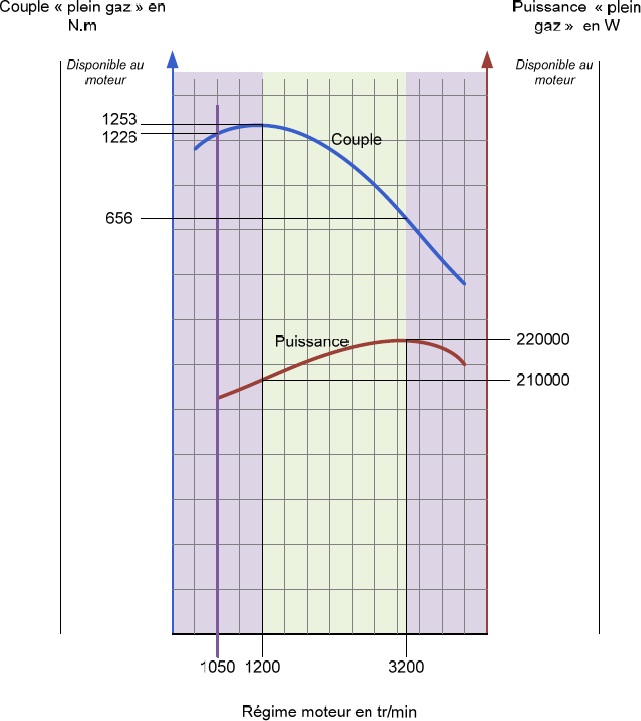
\includegraphics[width=.45\linewidth]{fig_19.png}
\caption{Acquisition de l’orientation des roues directrices \label{fig_19}}
\end{figure}


\begin{figure}[H]
\centering
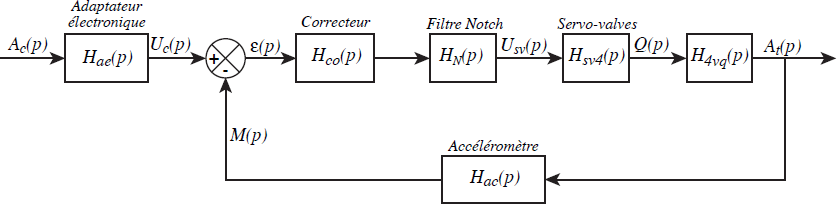
\includegraphics[width=.45\linewidth]{fig_20.png}
\caption{Schéma blocs de la commande en position des roues \label{fig_20}}
\end{figure}


\begin{figure}[H]
\centering
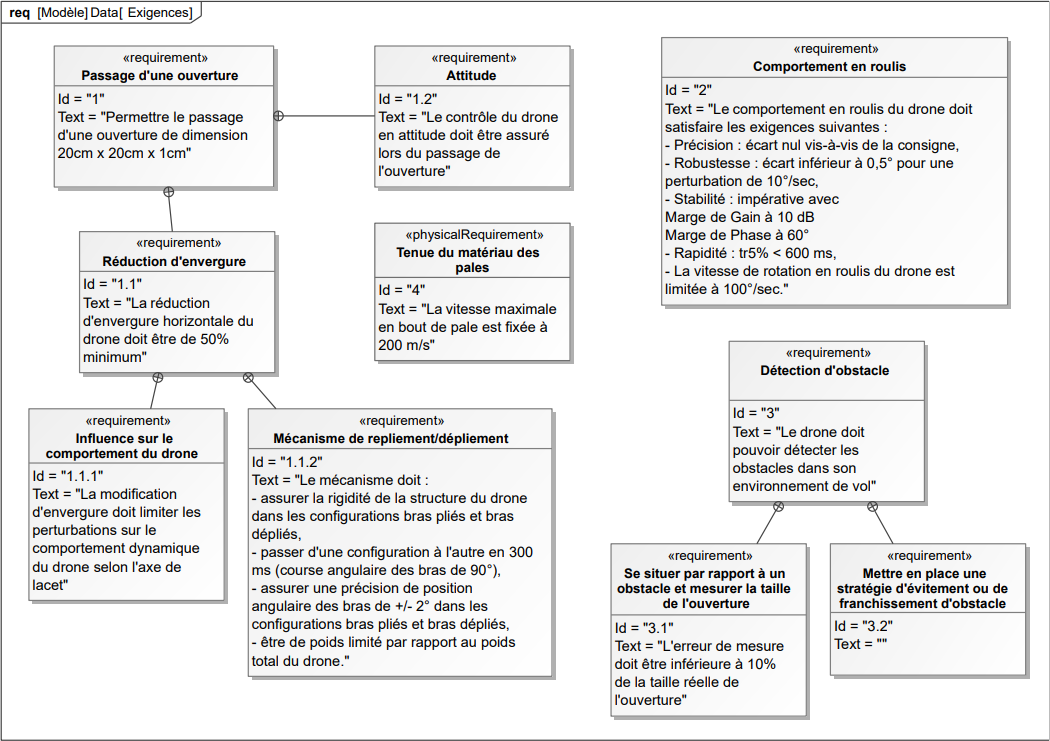
\includegraphics[width=.45\linewidth]{fig_21.png}
\caption{Évolution temporelle de $\alpha(t)$ pour une correction proportionnelle \label{fig_21}}
\end{figure}


\begin{figure}[H]
\centering
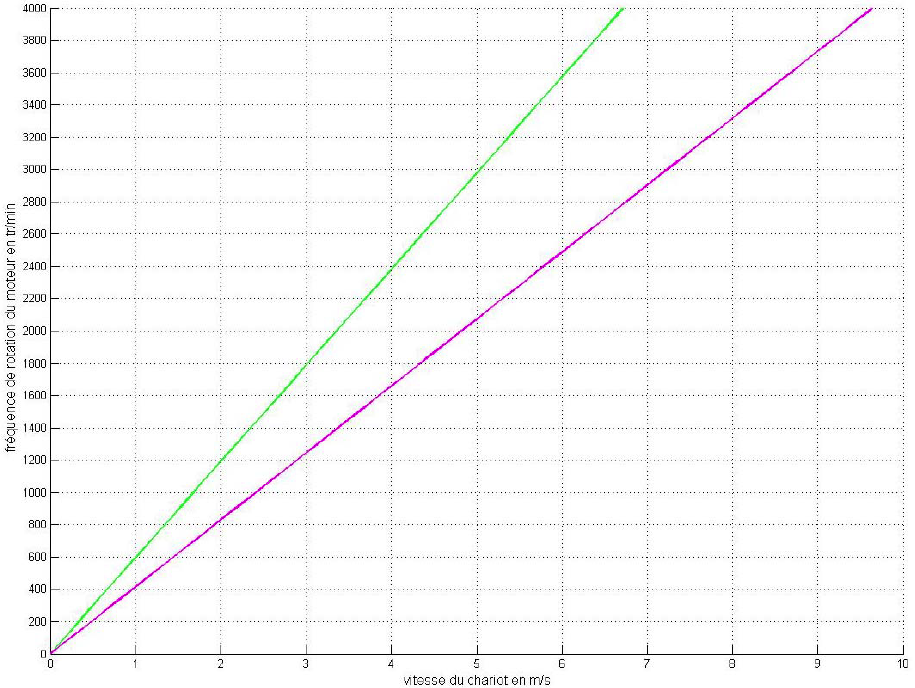
\includegraphics[width=.45\linewidth]{fig_22.png}
\caption{Essais expérimentaux réalisés sur le véhicule RC \label{fig_22}}
\end{figure}


\begin{figure}[H]
\centering
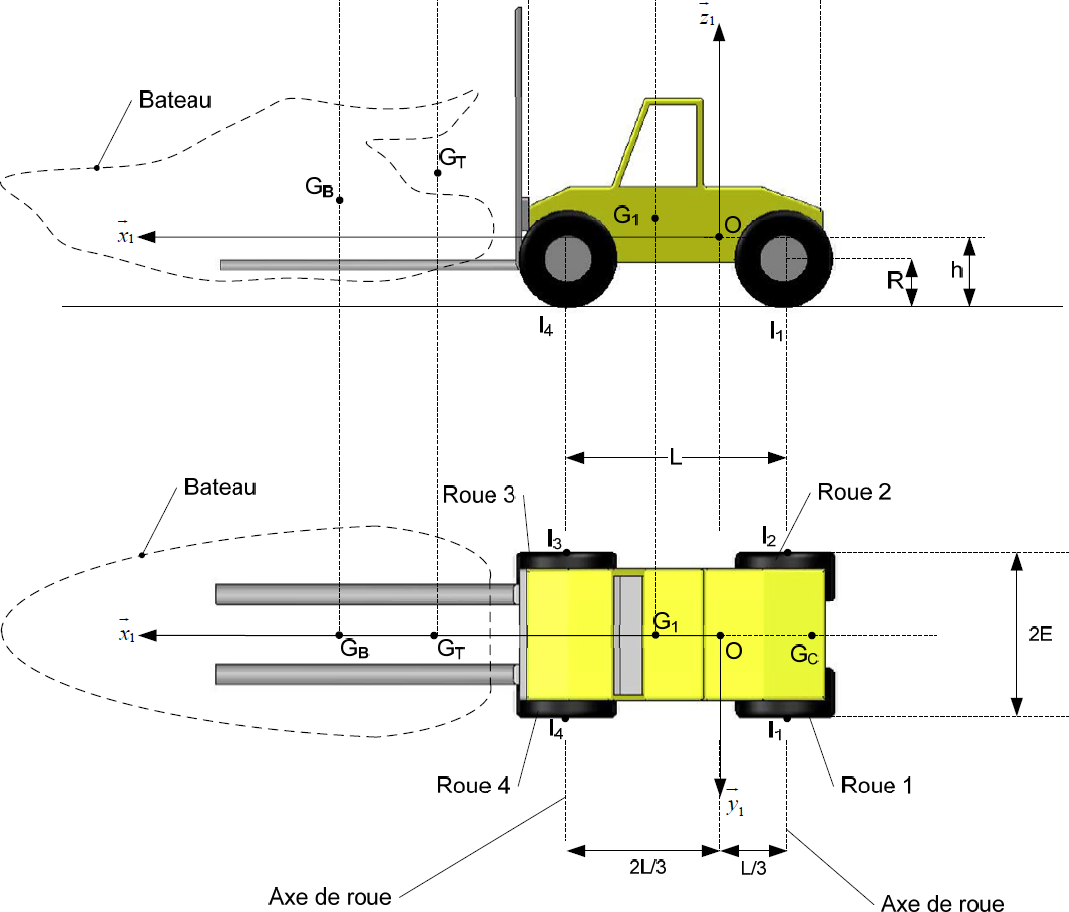
\includegraphics[width=.45\linewidth]{fig_23.png}
\caption{Diagrammes de Bode de la FTBO corrigée \label{fig_23}}
\end{figure}


\begin{figure}[H]
\centering
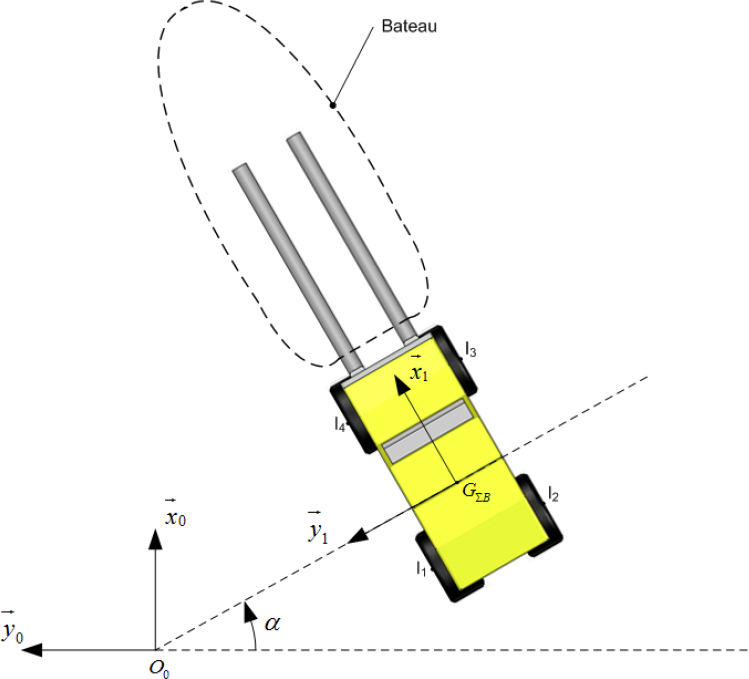
\includegraphics[width=.45\linewidth]{fig_24.png}
\caption{Angle des roues directrices \label{fig_24}}
\end{figure}


\begin{figure}[H]
\centering
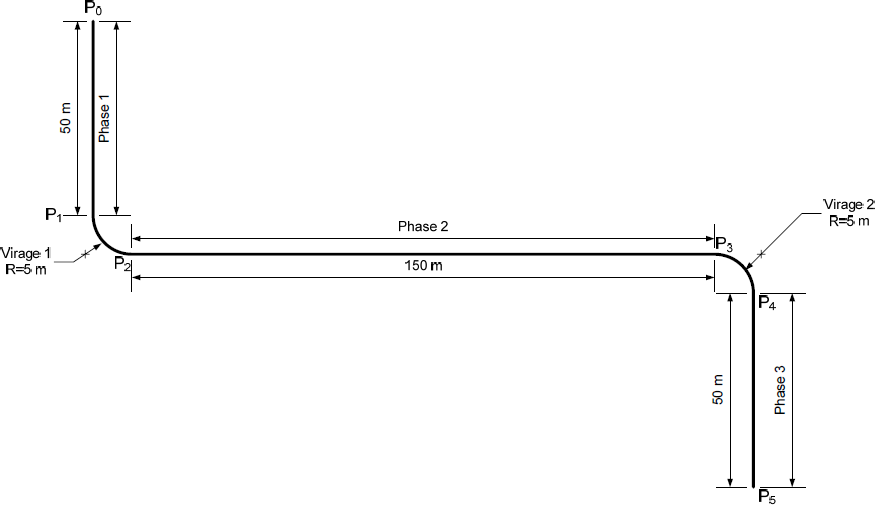
\includegraphics[width=.45\linewidth]{fig_25.png}
\caption{Résultat d’un essai de manoeuvre d’insertion avec l’algorithme d’aide au stationnement \label{fig_25}}
\end{figure}


\begin{figure}[H]
\centering
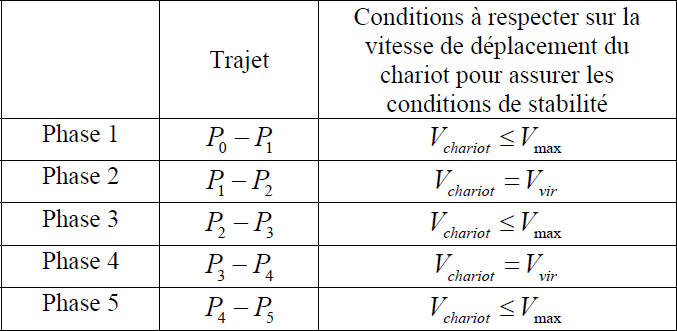
\includegraphics[width=.45\linewidth]{fig_26.png}
\caption{Extrait du diagramme des exigences du stationnement automatique \label{fig_26}}
\end{figure}


\begin{figure}[H]
\centering
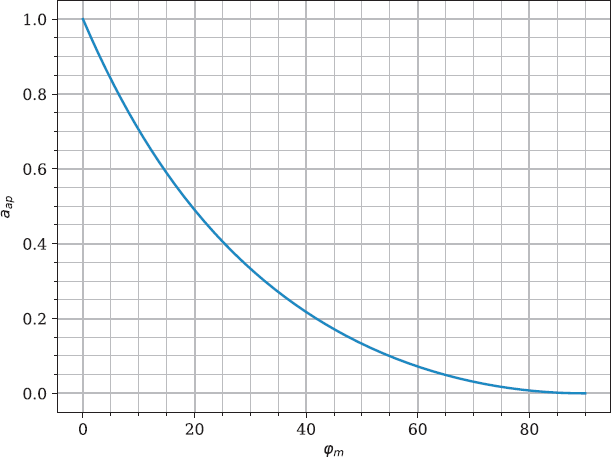
\includegraphics[width=.45\linewidth]{fig_27.png}
\caption{Extrait du diagramme des exigences du stationnement automatique \label{fig_27}}
\end{figure}


\begin{figure}[H]
\centering
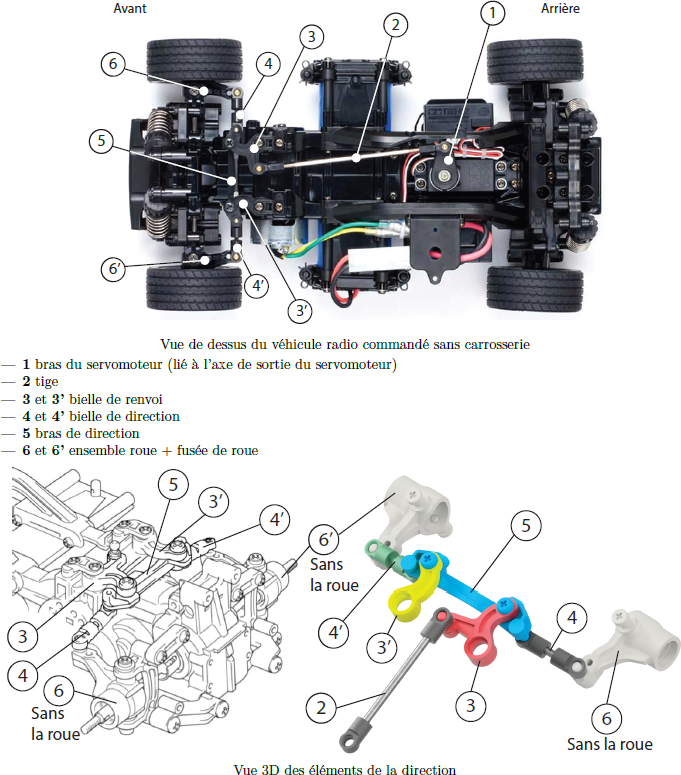
\includegraphics[width=.45\linewidth]{fig_28.png}
\caption{Description de la direction du véhicule radio commandé \label{fig_28}}
\end{figure}


\begin{figure}[H]
\centering
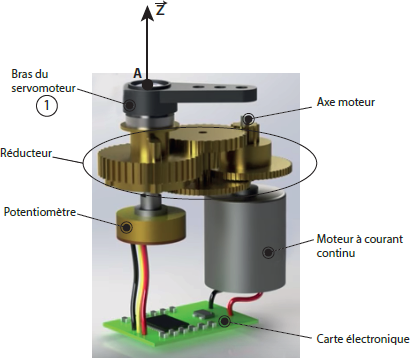
\includegraphics[width=.45\linewidth]{fig_29.png}
\caption{Composition du servomoteur \label{fig_29}}
\end{figure}